\chapter{Integrales triples}

\section*{Introducción}

Las integrales dobles permiten sumar valores de una función sobre regiones planas y calcular áreas, masas de láminas y momentos de inercia en dos dimensiones. Al pasar al espacio tridimensional, la misma idea se extiende de manera natural: ahora sumamos sobre sólidos, y el elemento de volumen es un pequeño paralelepípedo \(\Delta V = \Delta x\,\Delta y\,\Delta z\). Este proceso conduce a la \textbf{integral triple}, que es la herramienta fundamental para calcular volúmenes, masas de cuerpos con densidad variable, centros de masa y momentos de inercia en el espacio.

El hilo conductor de esta lección es el mismo que en las integrales dobles: \emph{particionar, aproximar y tomar el límite}. La novedad es que ahora la partición es tridimensional y la región de integración es un sólido. El Teorema de Fubini (marcado con asterisco en el programa de la asignatura) garantiza que la integral triple puede evaluarse mediante integrales iteradas en cualquiera de los seis órdenes posibles, siempre que los límites se ajusten correctamente a la geometría del sólido. En esta lección estudiaremos las coordenadas rectangulares y su extensión a las coordenadas cilíndricas y esféricas, herramientas que simplifican enormemente el cálculo sobre sólidos con simetría axial o esférica.

\section{Integrales triples en coordenadas rectangulares}

\begin{definition}[Integral triple]
Sea \(D\) una región cerrada y acotada en \(\mathbb{R}^3\), y sea \(f(x,y,z)\) una función continua en \(D\). Dividimos \(D\) en \(n\) subregiones (cajas) de volumen \(\Delta V_k\), elegimos un punto \((x_k^*, y_k^*, z_k^*)\) en cada subregión y formamos la suma de Riemann
\[
S_n = \sum_{k=1}^{n} f(x_k^*, y_k^*, z_k^*)\,\Delta V_k.
\]
Si el límite
\[
\lim_{\|P\| \to 0} S_n
\]
existe, donde \(\|P\|\) es la norma de la partición (el máximo diámetro de las subregiones), entonces dicho límite se denomina \textbf{integral triple} de \(f\) sobre \(D\) y se denota
\[
\iiint_D f(x,y,z)\,dV
\quad\text{o bien}\quad
\iiint_D f(x,y,z)\,dx\,dy\,dz.
\]
\end{definition}

Geométricamente, si \(f\equiv 1\), la integral triple da el volumen del sólido \(D\). Si \(f\) representa una densidad de masa, la integral triple da la masa total.

\begin{theorem}[Teorema de Fubini para integrales triples] \label{th:fubini3d}
Sea \(D\) una región sólida acotada en \(\mathbb{R}^3\) y sea \(f\) continua en \(D\). Entonces la integral triple de \(f\) sobre \(D\) puede calcularse como una integral iterada en cualquiera de los seis órdenes posibles. Por ejemplo, si la proyección de \(D\) sobre el plano \(xy\) es \(R\), y para cada \((x,y)\in R\) la variable \(z\) varía entre \(z_1(x,y)\) y \(z_2(x,y)\), entonces
\[
\iiint_D f(x,y,z)\,dV
=
\int_{x=a}^{b}\int_{y=g_1(x)}^{g_2(x)}
\int_{z=z_1(x,y)}^{z_2(x,y)}
f(x,y,z)\,dz\,dy\,dx,
\]
donde los límites exteriores describen la región \(R\).
\end{theorem}

\begin{rem}
El Teorema de Fubini es el fundamento que permite evaluar integrales triples mediante tres integraciones sucesivas. La elección del orden de integración no altera el valor de la integral, pero una elección adecuada puede simplificar enormemente los límites y los cálculos. En esta lección trabajaremos principalmente con el orden \(dz\,dy\,dx\), pero es importante recordar que los otros cinco órdenes son igualmente válidos. El cambio de orden, cuando se necesita, exige reexpresar la región \(D\) con los nuevos límites; lo ilustraremos con un ejemplo.
\end{rem}

\subsection*{Protocolo para evaluar integrales triples en coordenadas rectangulares}

Para montar y evaluar una integral triple sobre un sólido \(D\), se puede seguir el siguiente procedimiento.

\begin{pasos}[Evaluación de una integral triple en coordenadas rectangulares]
\begin{enumerate}
    \item \textbf{Identificar el sólido \(D\):} describir las superficies que lo limitan y, si es posible, dibujar un esquema.
    \item \textbf{Elegir el orden de integración:} decidir, por ejemplo, \(dz\,dy\,dx\). La elección depende de la geometría y de la facilidad para integrar la función.
    \item \textbf{Proyectar el sólido sobre el plano de las variables externas:} si se integra primero \(z\), proyectar \(D\) sobre el plano \(xy\); la proyección es una región \(R\) en el plano.
    \item \textbf{Determinar los límites de la variable interna:} para cada punto \((x,y)\) en \(R\), la variable \(z\) varía entre una superficie inferior \(z = z_1(x,y)\) y una superior \(z = z_2(x,y)\).
    \item \textbf{Determinar los límites de la variable intermedia:} para cada valor fijo de la variable externa (por ejemplo \(x\)), la variable intermedia \(y\) varía entre dos curvas que delimitan la proyección \(R\): \(y = g_1(x)\) y \(y = g_2(x)\).
    \item \textbf{Determinar los límites de la variable externa:} los valores extremos de la variable externa, digamos \(a \le x \le b\).
    \item \textbf{Escribir la integral iterada:}
    \[
    \iiint_D f\,dV =
    \int_{x=a}^{b}
    \int_{y=g_1(x)}^{g_2(x)}
    \int_{z=z_1(x,y)}^{z_2(x,y)}
    f(x,y,z)\,dz\,dy\,dx.
    \]
    \item \textbf{Evaluar paso a paso:} primero integrar respecto a \(z\), luego respecto a \(y\) y finalmente respecto a \(x\).
\end{enumerate}
\end{pasos}

\begin{rem}
El paso 5 puede variar según el orden elegido. Si se integra primero \(z\), la proyección es sobre \(xy\); si se integra primero \(y\), la proyección es sobre \(xz\), etc. La clave es siempre mantener fija la variable externa al describir los límites de la variable intermedia.
\end{rem}

\section{Ejemplos}

\begin{example}[Volumen de un tetraedro]
Calcular el volumen del sólido \(D\) limitado por los planos coordenados \(x=0\), \(y=0\), \(z=0\) y el plano \(x+y+z=1\).
\begin{myproof}
Seguimos los pasos del protocolo.

\begin{enumerate}
    \item \textbf{Identificar el sólido:} \(D\) es el tetraedro con vértices \((0,0,0)\), \((1,0,0)\), \((0,1,0)\) y \((0,0,1)\).
    \item \textbf{Elegir orden:} \(dz\,dy\,dx\).
    \item \textbf{Proyectar sobre \(xy\):} la proyección \(R\) es el triángulo \(x\ge0\), \(y\ge0\), \(x+y\le1\).
    \item \textbf{Límites de \(z\):} para \((x,y)\in R\), \(z\) varía desde \(z=0\) hasta \(z=1-x-y\).
    \item \textbf{Límites de \(y\):} para \(x\) fijo, \(y\) varía desde \(0\) hasta \(1-x\).
    \item \textbf{Límites de \(x\):} \(x\) varía desde \(0\) hasta \(1\).
    \item \textbf{Integral iterada:}
    \[
    V = \int_{0}^{1}\int_{0}^{1-x}\int_{0}^{1-x-y} dz\,dy\,dx.
    \]
    \item \textbf{Evaluar:}
    \[
    \int_{0}^{1-x-y} dz = 1-x-y,
    \]
    luego
    \[
    V = \int_{0}^{1}\int_{0}^{1-x} (1-x-y)\,dy\,dx.
    \]
    La integral interior:
    \[
    \int_{0}^{1-x} (1-x-y)\,dy
    = \left[(1-x)y - \frac{y^2}{2}\right]_{0}^{1-x}
    = (1-x)^2 - \frac{(1-x)^2}{2}
    = \frac{(1-x)^2}{2}.
    \]
    Finalmente,
    \[
    V = \int_{0}^{1} \frac{(1-x)^2}{2}\,dx
    = \frac{1}{2}\left[-\frac{(1-x)^3}{3}\right]_{0}^{1}
    = \frac{1}{2}\cdot\frac{1}{3} = \frac{1}{6}.
    \]
    Por tanto, \(\boxed{V = \frac{1}{6}}\).
\end{enumerate}
\end{myproof}
\end{example}

\begin{example}[Integral de una función sobre el tetraedro]
Calcular \(\iiint_D (x+y)\,dV\), donde \(D\) es el mismo tetraedro del ejemplo anterior.
\begin{myproof}
\textbf{Paso 1. Plantear la integral.} Usamos el mismo orden y los mismos límites. La integral es
\[
I = \int_{0}^{1}\int_{0}^{1-x}\int_{0}^{1-x-y} (x+y)\,dz\,dy\,dx.
\]
\textbf{Paso 2. Integrar en $z$.}
\[
\int_{0}^{1-x-y} (x+y)\,dz = (x+y)(1-x-y).
\]
Luego,
\[
I = \int_{0}^{1}\int_{0}^{1-x} (x+y)(1-x-y)\,dy\,dx.
\]
\textbf{Paso 3. Integral interior (cambio $u=x+y$).} Cuando \(y=0\), \(u=x\); cuando \(y=1-x\), \(u=1\). Entonces \(dy=du\) y
\[
\int_{0}^{1-x} (x+y)(1-x-y)\,dy
= \int_{x}^{1} u(1-u)\,du
= \left[\frac{u^2}{2} - \frac{u^3}{3}\right]_{x}^{1}
= \frac{1}{6} - \frac{x^2}{2} + \frac{x^3}{3}.
\]
\textbf{Paso 4. Integrar en $x$.}
\[
I = \int_{0}^{1} \left(\frac{1}{6} - \frac{x^2}{2} + \frac{x^3}{3}\right) dx
= \left[\frac{x}{6} - \frac{x^3}{6} + \frac{x^4}{12}\right]_{0}^{1}
= \frac{1}{6} - \frac{1}{6} + \frac{1}{12}
= \frac{1}{12}.
\]
Por tanto, \(\boxed{\iiint_D (x+y)\,dV = \frac{1}{12}}\).
\end{myproof}
\end{example}

\begin{example}[Volumen de un sólido bajo un paraboloide]
Calcular el volumen del sólido \(D\) encerrado entre el paraboloide \(z = x^2 + y^2\) y el plano \(z = 0\), sobre el cuadrado \(0 \le x \le 1\), \(0 \le y \le 1\).
\begin{myproof}
\textbf{Paso 1. Plantear la integral triple.} El sólido se proyecta sobre el cuadrado \(R = [0,1]\times[0,1]\). Para cada \((x,y)\in R\), \(z\) varía desde \(0\) hasta \(x^2+y^2\). Elegimos el orden \(dz\,dy\,dx\).

\[
V = \int_{0}^{1}\int_{0}^{1}\int_{0}^{x^2+y^2} dz\,dy\,dx
= \int_{0}^{1}\int_{0}^{1} (x^2+y^2)\,dy\,dx.
\]
\textbf{Paso 2. Integrar en $y$.}
\[
\int_{0}^{1} (x^2+y^2)\,dy = x^2 + \frac{1}{3}.
\]
\textbf{Paso 3. Integrar en $x$.}
\[
V = \int_{0}^{1} \left(x^2 + \frac{1}{3}\right) dx
= \frac{1}{3} + \frac{1}{3} = \frac{2}{3}.
\]
Por tanto, \(\boxed{V = \frac{2}{3}}\).
\end{myproof}
\end{example}

\begin{example}[Cambio de orden de integración (tema con asterisco)]
Dada la integral
\[
I = \int_{0}^{1}\int_{0}^{x}\int_{0}^{x+y} f(x,y,z)\,dz\,dy\,dx,
\]
reescribirla en el orden \(dz\,dx\,dy\).
\begin{myproof}
\textbf{Paso 1. Identificar el sólido.} Observamos los límites del orden original: \(x\) entre \(0\) y \(1\), para cada \(x\), \(y\) entre \(0\) y \(x\), y para cada \((x,y)\), \(z\) entre \(0\) y \(x+y\). Esto describe el sólido
\[
D = \{ (x,y,z) : 0 \le x \le 1,\; 0 \le y \le x,\; 0 \le z \le x+y \}.
\]
\textbf{Paso 2. Nuevo orden $dz\,dx\,dy$.} Queremos integrar primero \(z\), luego \(x\), luego \(y\). Para ello, necesitamos describir \(D\) en el orden \(dz\,dx\,dy\): fijamos \(y\), luego \(x\) varía entre ciertos límites dependiendo de \(y\), y finalmente \(y\) varía entre valores constantes.

De las condiciones originales, \(0 \le y \le x \le 1\), así que \(y\) varía entre \(0\) y \(1\). Para \(y\) fijo, \(x\) varía entre \(y\) y \(1\). Para cada \((x,y)\), \(z\) varía entre \(0\) y \(x+y\). Por tanto, la integral reescrita es
\[
\boxed{I = \int_{y=0}^{1}\int_{x=y}^{1}\int_{z=0}^{x+y} f(x,y,z)\,dz\,dx\,dy.}
\]
Este es un ejemplo de cómo el cambio de orden requiere reexpresar cuidadosamente las desigualdades que definen el sólido.
\end{myproof}
\end{example}

\section{Masa, centros de masa y momentos de inercia}

Las integrales triples son la herramienta natural para calcular propiedades físicas de cuerpos tridimensionales con densidad variable \(\rho(x,y,z)\). La masa total, el centro de masa y los momentos de inercia se obtienen como integrales de la densidad o de sus productos con las coordenadas.

\subsection{Masa total}

Si \(\rho(x,y,z)\) es la densidad (masa por unidad de volumen) de un sólido \(D\), la masa total es
\[
M = \iiint_D \rho(x,y,z)\,dV.
\]

\subsection{Centro de masa}

El centro de masa \((\bar{x},\bar{y},\bar{z})\) se define mediante los primeros momentos respecto a los planos coordenados:
\[
M_{yz} = \iiint_D x\,\rho\,dV,\quad
M_{xz} = \iiint_D y\,\rho\,dV,\quad
M_{xy} = \iiint_D z\,\rho\,dV,
\]
y entonces
\[
\bar{x} = \frac{M_{yz}}{M},\quad
\bar{y} = \frac{M_{xz}}{M},\quad
\bar{z} = \frac{M_{xy}}{M}.
\]
Si la densidad es constante, el centro de masa coincide con el centroide del sólido.

\subsection{Momentos de inercia}

El momento de inercia mide la resistencia de un cuerpo a la rotación alrededor de un eje. Para un eje \(L\), el momento de inercia es
\[
I_L = \iiint_D r_{\perp}^2\,\rho\,dV,
\]
donde \(r_{\perp}\) es la distancia desde el punto \((x,y,z)\) al eje \(L\). En coordenadas cartesianas, los momentos de inercia respecto a los ejes \(x\), \(y\) y \(z\) son:
\[
I_x = \iiint_D (y^2+z^2)\,\rho\,dV,\quad
I_y = \iiint_D (x^2+z^2)\,\rho\,dV,\quad
I_z = \iiint_D (x^2+y^2)\,\rho\,dV.
\]

\begin{rem}
El momento de inercia es análogo a la masa en el movimiento lineal: así como la masa mide la inercia frente a cambios de velocidad lineal, el momento de inercia mide la inercia frente a cambios de velocidad angular. Las integrales triples permiten calcular estos momentos para cuerpos de forma arbitraria y densidad variable.
\end{rem}

\subsection{Ejemplos de aplicaciones físicas}

\begin{example}[Masa y centro de masa con densidad constante]
Calcular la masa y el centro de masa del tetraedro del ejemplo 1, si la densidad es constante \(\rho = k\).
\begin{myproof}
\textbf{Paso 1. Masa.}
La masa es
\[
M = \iiint_D k\,dV = k\,V = \frac{k}{6}.
\]
\textbf{Paso 2. Centro de masa (argumento de simetría).} Por simetría del tetraedro con respecto a las tres coordenadas, el centro de masa se encuentra en \((\bar{x},\bar{y},\bar{z}) = (1/4,1/4,1/4)\). Verifiquemos, por ejemplo, \(\bar{x}\):
\[
\bar{x} = \frac{1}{M}\iiint_D x\,k\,dV = \frac{1}{V}\iiint_D x\,dV.
\]
\textbf{Paso 3. Calcular $\iiint_D x\,dV$.}
\[
\int_{0}^{1}\int_{0}^{1-x}\int_{0}^{1-x-y} x\,dz\,dy\,dx
= \int_{0}^{1}\int_{0}^{1-x} x(1-x-y)\,dy\,dx
= \int_{0}^{1} x\left[(1-x)^2 - \frac{(1-x)^2}{2}\right] dx
= \frac{1}{2}\int_{0}^{1} x(1-x)^2 dx.
\]
La integral \(\int_{0}^{1} x(1-x)^2 dx = \int_{0}^{1} (x - 2x^2 + x^3) dx = \frac12 - \frac23 + \frac14 = \frac{1}{12}\). Por tanto,
\[
\iiint_D x\,dV = \frac12\cdot\frac{1}{12} = \frac{1}{24}.
\]
Entonces \(\bar{x} = \frac{1/24}{1/6} = \frac14\). Análogamente \(\bar{y}=\bar{z}=1/4\). \(\boxed{M = k/6,\; (\bar{x},\bar{y},\bar{z}) = (1/4,1/4,1/4)}\).
\end{myproof}
\end{example}

\begin{example}[Masa con densidad variable]
Sea \(D\) el tetraedro del ejemplo 1 y sea \(\rho(x,y,z) = xyz\). Calcular la masa total.
\begin{myproof}
\[
M = \iiint_D xyz\,dV
= \int_{0}^{1}\int_{0}^{1-x}\int_{0}^{1-x-y} xyz\,dz\,dy\,dx.
\]
\textbf{Paso 1. Integrar en $z$.}
\[
\int_{0}^{1-x-y} xyz\,dz = xy\,\frac{(1-x-y)^2}{2}.
\]
\textbf{Paso 2. Integral doble resultante.}
\[
M = \frac12\int_{0}^{1}\int_{0}^{1-x} xy(1-x-y)^2\,dy\,dx.
\]
\textbf{Paso 3. Integral interior (sustitución).}
\[
\int_{0}^{1-x} y(1-x-y)^2\,dy.
\]
Hacemos \(u = 1-x-y\), entonces \(y = 1-x-u\), \(dy = -du\). Cuando \(y=0\), \(u=1-x\); cuando \(y=1-x\), \(u=0\). La integral se convierte en
\[
\int_{1-x}^{0} (1-x-u)u^2(-du) = \int_{0}^{1-x} (1-x-u)u^2\,du
= (1-x)\int_{0}^{1-x} u^2\,du - \int_{0}^{1-x} u^3\,du
= (1-x)\frac{(1-x)^3}{3} - \frac{(1-x)^4}{4}
= \frac{(1-x)^4}{12}.
\]
\textbf{Paso 4. Resultado final.}
\[
M = \frac12\int_{0}^{1} x\cdot \frac{(1-x)^4}{12}\,dx
= \frac{1}{24}\int_{0}^{1} x(1-x)^4\,dx.
\]
La integral \(\int_{0}^{1} x(1-x)^4 dx = \frac{1}{30}\) (usando la fórmula beta o integrando por partes). Entonces
\[
M = \frac{1}{24}\cdot\frac{1}{30} = \frac{1}{720}.
\]
\(\boxed{M = \frac{1}{720}}\).
\end{myproof}
\end{example}

\begin{example}[Momento de inercia respecto al eje \(z\)]
Calcular \(I_z\) para el cubo \(D = [0,1]^3\) con densidad constante \(\rho = 1\).
\begin{myproof}
\[
I_z = \iiint_D (x^2+y^2)\,dV
= \int_{0}^{1}\int_{0}^{1}\int_{0}^{1} (x^2+y^2)\,dz\,dy\,dx.
\]
\textbf{Paso 1. Integrar en $z$.}
\[
\int_{0}^{1} (x^2+y^2)\,dz = x^2+y^2.
\]
\textbf{Paso 2. Integrar la doble integral.}
\[
I_z = \int_{0}^{1}\int_{0}^{1} (x^2+y^2)\,dy\,dx
= \int_{0}^{1} \left[x^2 y + \frac{y^3}{3}\right]_{0}^{1} dx
= \int_{0}^{1} \left(x^2 + \frac13\right) dx
= \frac13 + \frac13 = \frac23.
\]
\(\boxed{I_z = \frac{2}{3}}\).
\end{myproof}
\end{example}

\section{Problemas propuestos}

\begin{prob}
Calcular el volumen del sólido limitado por los planos \(x=0\), \(x=1\), \(y=0\), \(y=1\), \(z=0\) y el plano \(z = 2 - x - y\).
\begin{myproof}
\textbf{Paso 1. Integral iterada.} El sólido es $0\le x\le1$, $0\le y\le1$, $0\le z\le 2-x-y$ (la cota es positiva pues $x+y\le2$ en la región). Orden $dz\,dy\,dx$:
\[
V = \int_0^1\int_0^1\int_0^{2-x-y} dz\,dy\,dx.
\]
\textbf{Paso 2. Integrar en $z$.}
\[
\int_0^{2-x-y} dz = 2-x-y.
\]
\textbf{Paso 3. Integrar en $y$.}
\[
\int_0^1(2-x-y)\,dy
= \Bigl[2y-xy-\tfrac{y^2}{2}\Bigr]_0^1 = \tfrac{3}{2}-x.
\]
\textbf{Paso 4. Integrar en $x$.}
\[
V = \int_0^1\!\Bigl(\tfrac{3}{2}-x\Bigr)dx
= \Bigl[\tfrac{3x}{2}-\tfrac{x^2}{2}\Bigr]_0^1
= \tfrac{3}{2}-\tfrac{1}{2} = \boxed{1}.
\]
\end{myproof}
\end{prob}

\begin{prob}
Evaluar \(\iiint_D (x^2 + y^2 + z^2)\,dV\), donde \(D\) es el cubo \([0,1]^3\).
\end{prob}

\begin{prob}
Calcular el volumen del sólido encerrado entre el cilindro \(x^2+y^2=1\) y los planos \(z=0\) y \(z=2\) (sugerencia: usar coordenadas rectangulares, proyectar sobre el círculo unidad).
\end{prob}

\begin{prob}
Sea \(D\) el sólido limitado por \(z=0\), \(z=4-x^2-y^2\) y el cilindro \(x^2+y^2=4\). Calcular su volumen. (Nota: la proyección es el disco \(x^2+y^2\le4\); los límites en \(x\) e \(y\) son \(-2\le x\le2\), \(-\sqrt{4-x^2}\le y\le\sqrt{4-x^2}\).)
\end{prob}

\begin{prob}
Reescribir la integral
\[
\int_{0}^{1}\int_{0}^{1}\int_{0}^{y} f(x,y,z)\,dz\,dy\,dx
\]
en el orden \(dz\,dx\,dy\).
\end{prob}

\begin{prob}
Un sólido \(D\) ocupa la región limitada por \(x=0\), \(x=2\), \(y=0\), \(y=3\), \(z=0\) y \(z=5\). Su densidad es \(\rho(x,y,z) = xyz\). Calcular la masa total.
\begin{myproof}
\textbf{Paso 1. Plantear.}
\[
M = \int_0^2\int_0^3\int_0^5 xyz\,dz\,dy\,dx.
\]
\textbf{Paso 2. Integrar en $z$.}
\[
\int_0^5 xyz\,dz = xy\cdot\frac{z^2}{2}\Big|_0^5 = \frac{25xy}{2}.
\]
\textbf{Paso 3. Integrar en $y$.}
\[
\int_0^3 \frac{25xy}{2}\,dy = \frac{25x}{2}\cdot\frac{y^2}{2}\Big|_0^3 = \frac{225x}{4}.
\]
\textbf{Paso 4. Integrar en $x$.}
\[
M = \int_0^2 \frac{225x}{4}\,dx
= \frac{225}{4}\cdot\frac{x^2}{2}\Big|_0^2 = \frac{225}{4}\cdot 2 = \boxed{\dfrac{225}{2}}.
\]
\end{myproof}
\end{prob}

\begin{prob}
Para el tetraedro del ejemplo 1, con densidad constante \(\rho=1\), calcular \(I_x = \iiint_D (y^2+z^2)\,dV\).
\end{prob}

\begin{prob}
Sea \(D\) el sólido bajo el paraboloide \(z=x^2+y^2\) y sobre el cuadrado \([0,1]\times[0,1]\) (ejemplo 3). Calcular la masa si la densidad es \(\rho(x,y,z) = x\).
\end{prob}

\begin{prob}
Encontrar el centro de masa del sólido \(D = \{ (x,y,z): 0\le x\le1,\;0\le y\le1,\;0\le z\le x+y \}\) con densidad constante \(\rho=1\).
\end{prob}

\begin{prob}
Calcular \(I_z\) para el tetraedro del ejemplo 1 con densidad constante \(\rho=1\).
\end{prob}

\begin{rem}
Los problemas marcados con asterisco son de carácter no exigente en la evaluación coordinada, pero se incluyen para completar la formación.
\end{rem}

% ============================================================
\section{Coordenadas cilíndricas}
% ============================================================

Las \textbf{coordenadas cilíndricas} $(r,\theta,z)$ generalizan las coordenadas polares al espacio: $x$ e $y$ se expresan en términos de $r$ y $\theta$, mientras que $z$ permanece igual.

\begin{definition}[Coordenadas cilíndricas]
Las coordenadas cilíndricas $(r,\theta,z)$ se relacionan con las coordenadas rectangulares $(x,y,z)$ mediante
\[
x = r\cos\theta,\quad y = r\sen\theta,\quad z = z,
\quad r\ge0,\;\theta\in[0,2\pi).
\]
El jacobiano de la transformación es $r$, por lo que el elemento de volumen es
\[
dV = r\,dr\,d\theta\,dz.
\]
\end{definition}

\begin{theorem}[Integral triple en coordenadas cilíndricas]
Si el sólido $D$ se describe como $\alpha\le\theta\le\beta$, $g_1(\theta)\le r\le g_2(\theta)$, $z_1(r,\theta)\le z\le z_2(r,\theta)$, entonces
\[
\iiint_D f(x,y,z)\,dV
= \int_{\alpha}^{\beta}\int_{g_1(\theta)}^{g_2(\theta)}\int_{z_1}^{z_2}
  f(r\cos\theta,\, r\sen\theta,\, z)\;r\,dz\,dr\,d\theta.
\]
\end{theorem}

\subsection*{Protocolo para integrales triples en coordenadas cilíndricas}

\begin{pasos}[Evaluación en coordenadas cilíndricas]
\begin{enumerate}
    \item \textbf{Identificar simetría axial:} si la proyección sobre $xy$ tiene forma circular o anular, usar coordenadas cilíndricas.
    \item \textbf{Reescribir la región:} sustituir $x=r\cos\theta$, $y=r\sen\theta$ en las ecuaciones de las superficies para obtener los límites de $z$ en función de $r,\theta$.
    \item \textbf{Determinar los límites radiales $r$ y angulares $\theta$} de la proyección circular.
    \item \textbf{Escribir e integrar:}
    \[
    \iiint_D f\,dV = \int_{\alpha}^{\beta}\int_{r_1(\theta)}^{r_2(\theta)}\int_{z_1(r,\theta)}^{z_2(r,\theta)}
    f(r\cos\theta,r\sen\theta,z)\;r\,dz\,dr\,d\theta.
    \]
\end{enumerate}
\end{pasos}

\begin{example}[Volumen de un sólido con simetría cilíndrica]
Calcular el volumen del sólido acotado superiormente por el paraboloide $z=4-x^2-y^2$ e inferiormente por $z=0$, dentro del cilindro $x^2+y^2=4$.
\begin{myproof}
\textbf{Paso 1. Describir el sólido en cilíndricas.} El cilindro $x^2+y^2=4$ es $r=2$. El paraboloide $z=4-x^2-y^2$ es $z=4-r^2$. Para $r\in[0,2]$ se tiene $4-r^2\ge0$, luego $z\in[0,4-r^2]$.

\textbf{Paso 2. Plantear la integral.}
\[
V = \int_{0}^{2\pi}\int_{0}^{2}\int_{0}^{4-r^2} r\,dz\,dr\,d\theta.
\]

\textbf{Paso 3. Integrar en $z$.}
\[
\int_{0}^{4-r^2} r\,dz = r(4-r^2),
\]
luego $V = \displaystyle\int_{0}^{2\pi}d\theta \cdot \int_{0}^{2} r(4-r^2)\,dr = 2\pi\int_{0}^{2}(4r-r^3)\,dr$.

\textbf{Paso 4. Integrar en $r$.}
\[
\int_{0}^{2}(4r-r^3)\,dr = \left[2r^2 - \frac{r^4}{4}\right]_{0}^{2} = 8-4 = 4.
\]
$\displaystyle\boxed{V = 2\pi\cdot 4 = 8\pi}$.
\end{myproof}
\end{example}

% ============================================================
\section{Coordenadas esféricas}
% ============================================================

Las \textbf{coordenadas esféricas} $(\rho,\varphi,\theta)$ son especialmente útiles cuando el sólido tiene simetría esférica o cónica.

\begin{definition}[Coordenadas esféricas]
Las coordenadas esféricas $(\rho,\varphi,\theta)$ se relacionan con las coordenadas rectangulares $(x,y,z)$ mediante
\[
x = \rho\sen\varphi\cos\theta,\quad
y = \rho\sen\varphi\sen\theta,\quad
z = \rho\cos\varphi,
\]
con $\rho\ge0$, $\varphi\in[0,\pi]$ y $\theta\in[0,2\pi)$. Nótese que $\rho^2 = x^2+y^2+z^2$.  El jacobiano es $\rho^2\sen\varphi$, por lo que el elemento de volumen es
\[
dV = \rho^2\sen\varphi\,d\rho\,d\varphi\,d\theta.
\]
\end{definition}

\begin{theorem}[Integral triple en coordenadas esféricas]
Si $D$ se describe como $\alpha\le\theta\le\beta$, $\varphi_1\le\varphi\le\varphi_2$, $0\le\rho\le g(\varphi,\theta)$, entonces
\[
\iiint_D f\,dV
= \int_{\alpha}^{\beta}\int_{\varphi_1}^{\varphi_2}\int_{0}^{g(\varphi,\theta)}
  f(\rho\sen\varphi\cos\theta,\rho\sen\varphi\sen\theta,\rho\cos\varphi)\;
  \rho^2\sen\varphi\,d\rho\,d\varphi\,d\theta.
\]
\end{theorem}

\subsection*{Protocolo para integrales triples en coordenadas esféricas}

\begin{pasos}[Evaluación en coordenadas esféricas]
\begin{enumerate}
    \item \textbf{Identificar simetría esférica o cónica:} si la región involucra $x^2+y^2+z^2=R^2$ o conos, las esféricas simplifican los límites.
    \item \textbf{Reescribir la región:} sustituir $x,y,z$ en términos de $\rho,\varphi,\theta$ para obtener los límites de $\rho$.
    \item \textbf{Determinar los límites de $\varphi$ (ángulo polar desde el eje $z$) y $\theta$ (ángulo azimutal)}.
    \item \textbf{Escribir e integrar, recordando incluir el jacobiano $\rho^2\sen\varphi$:}
    \[
    \iiint_D f\,dV = \int_{\alpha}^{\beta}\int_{\varphi_1}^{\varphi_2}\int_{0}^{g}
    f(\cdots)\;\rho^2\sen\varphi\,d\rho\,d\varphi\,d\theta.
    \]
\end{enumerate}
\end{pasos}

\begin{example}[Volumen de una bola]
Verificar que el volumen de la bola $x^2+y^2+z^2\le a^2$ es $\dfrac{4}{3}\pi a^3$.
\begin{myproof}
\textbf{Paso 1. Describir en esféricas.} La bola es $0\le\rho\le a$, $0\le\varphi\le\pi$, $0\le\theta\le2\pi$.

\textbf{Paso 2. Plantear la integral.}
\[
V = \int_{0}^{2\pi}\int_{0}^{\pi}\int_{0}^{a}\rho^2\sen\varphi\,d\rho\,d\varphi\,d\theta.
\]

\textbf{Paso 3. Separar en tres integrales independientes.} Las tres integrales se factorizan:
\[
V = \left(\int_{0}^{2\pi}d\theta\right)\left(\int_{0}^{\pi}\sen\varphi\,d\varphi\right)\left(\int_{0}^{a}\rho^2\,d\rho\right).
\]

\textbf{Paso 4. Evaluar cada factor.}
\[
\int_{0}^{2\pi}d\theta = 2\pi,\qquad
\int_{0}^{\pi}\sen\varphi\,d\varphi = \bigl[-\cos\varphi\bigr]_{0}^{\pi} = 2,\qquad
\int_{0}^{a}\rho^2\,d\rho = \frac{a^3}{3}.
\]
$\displaystyle\boxed{V = 2\pi\cdot 2\cdot \frac{a^3}{3} = \frac{4\pi a^3}{3}}$.
\end{myproof}
\end{example}


% ============================================================
% Cap. 33 — Integrales múltiples
% 68 problemas unicos (11 pstricks convertidos a TikZ)
% ============================================================

% --- Subtema: Coordenadas cilíndricas (6 problemas) ---

% >>> LISTOS PARA INTEGRAR AHORA <<<

% [Original: líneas 1722-1726 | sin verificar | sin figura | 6 variante(s) de parámetro (se descartaron 5)]
\begin{prob}
Use coordenadas cilíndricas para evaluar la integral
\[ \displaystyle\int_{0}^{4}\int_{0}^{6}\int_{0}^{\sqrt{36-x^2}}\ \left(x^2+y^2\right)\ dy\ dx\ dz\]
Exprese claramente los límites de integración correspondientes y la solución de la integral.
\begin{myproof}
\textbf{Paso 1. Identificar la región.} La región en $xy$ es $x\ge0$, $0\le y\le\sqrt{36-x^2}$: el cuarto de disco (primer cuadrante) con $x^2+y^2\le36$. Pasamos a coordenadas cilíndricas: $x=r\cos\theta$, $y=r\sen\theta$, $dV=r\,dr\,d\theta\,dz$.

\textbf{Paso 2. Nuevos límites.} $\theta\in[0,\pi/2]$ (primer cuadrante), $r\in[0,6]$, $z\in[0,4]$. Además $x^2+y^2=r^2$.

\textbf{Paso 3. Integral en cilíndricas.}
\[
I = \int_0^4\!\int_0^{\pi/2}\!\int_0^6 r^2\cdot r\,dr\,d\theta\,dz
= \underbrace{\int_0^4 dz}_{4}\cdot
  \underbrace{\int_0^{\pi/2}d\theta}_{\pi/2}\cdot
  \underbrace{\int_0^6 r^3\,dr}_{324}.
\]

\textbf{Paso 4. Resultado.}
\[
\int_0^6 r^3\,dr = \frac{r^4}{4}\Big|_0^6 = \frac{1296}{4}=324.
\qquad
I = 4\cdot\frac{\pi}{2}\cdot 324 = \boxed{648\pi}.
\]
\end{myproof}
\end{prob}



% [Original: líneas 2335-2337 | solo respuesta final | sin figura | 3 variante(s) de parámetro (se descartaron 2)]
\begin{prob}
Use coordenadas cilíndricas para determinar el valor de la integral triple $$\displaystyle\int\int\int_{\Omega}z^2\sen\left( x^2+y^2 \right)\  dV,$$ donde $\Omega$ es la región $$\Omega=\left\lbrace (x,y,z)\in \mathbb{R}^3 : 1\leq x^2+y^2 \leq 4,\ x\geq 0,\ x\leq y \leq \sqrt{3}x,\ 0\leq z\leq 2 \right\rbrace.$$ \textbf{Respuesta:} $\approx 0.41677$.
\end{prob}

% [Original: líneas 2361-2363 | solo respuesta final | sin figura | 3 variante(s) de parámetro (se descartaron 2)]
\begin{prob}
Use coordenadas cilíndricas para determinar el valor de la integral triple $$\displaystyle\int\int\int_{\Omega}z\cos\left( x^2+y^2 \right)\ dV,$$ donde $\Omega$ es la región $$\Omega=\left\lbrace (x,y,z)\in \mathbb{R}^3 : 4\leq x^2+y^2 \leq 9,\  x\geq 0,\ \dfrac{(\sqrt{3})x}{3} \leq y \leq \sqrt{3}x,\ 0\leq z\leq 3 \right\rbrace.$$ \textbf{Respuesta:} $\approx 1.3771$.
\end{prob}

% [Original: líneas 2387-2389 | solo respuesta final | sin figura]
\begin{prob}
Use coordenadas cilíndricas para determinar el valor de la integral triple $$\displaystyle\int\int\int_{\Omega}z^2\cos\left( x^2+y^2 \right)\ dV,$$ donde $\Omega$ es la región $$\Omega=\left\lbrace (x,y,z)\in \mathbb{R}^3 : 9\leq x^2+y^2 \leq 16,\ x\geq 0,\ \dfrac{(\sqrt{3})x}{3}\leq y \leq x,\ 1\leq z\leq 3 \right\rbrace.$$ \textbf{Respuesta:} $\approx -0.79414$.
\end{prob}

% --- Subtema: Coordenadas esféricas (2 problemas) ---

% >>> LISTOS PARA INTEGRAR AHORA <<<

% [Original: líneas 2339-2341 | solo respuesta final | sin figura | 2 variante(s) de parámetro (se descartaron 1)]
\begin{prob}
Use coordenadas esféricas para determinar el valor de la integral triple $$\displaystyle\int\int\int_{\Omega}5z\  dV,$$ donde $\Omega$ es la región $$\Omega=\left\lbrace (x,y,z)\in \mathbb{R}^3 : x^2+y^2+z^2 \leq 4,\ z\geq 0,\ z^2\geq x^2+y^2 \right\rbrace.$$
\begin{myproof}
\textbf{Paso 1. Región en esféricas.} La esfera da $\rho\le2$. La condición del cono $z\ge\sqrt{x^2+y^2}$ equivale, en esféricas, a $\cos\varphi\ge\sen\varphi$, es decir $\varphi\le\pi/4$. Así: $\rho\in[0,2]$, $\varphi\in[0,\pi/4]$, $\theta\in[0,2\pi]$.

\textbf{Paso 2. Plantear.} Con $z=\rho\cos\varphi$ y $dV=\rho^2\sen\varphi\,d\rho\,d\varphi\,d\theta$:
\[
\iiint_\Omega 5z\,dV
= 5\int_0^{2\pi}\!\int_0^{\pi/4}\!\int_0^2
  \rho^3\cos\varphi\sen\varphi\,d\rho\,d\varphi\,d\theta.
\]

\textbf{Paso 3. Separar los tres factores.}
\[
= 5\underbrace{\int_0^{2\pi}d\theta}_{2\pi}
  \cdot\underbrace{\int_0^{\pi/4}\cos\varphi\sen\varphi\,d\varphi}_{I_\varphi}
  \cdot\underbrace{\int_0^2\rho^3\,d\rho}_{4}.
\]

\textbf{Paso 4. Calcular $I_\varphi$.} Usando $\cos\varphi\sen\varphi=\frac12\sen2\varphi$:
\[
I_\varphi = \frac12\!\int_0^{\pi/4}\!\sen2\varphi\,d\varphi
= \frac12\Bigl[-\frac{\cos2\varphi}{2}\Bigr]_0^{\pi/4}
= \frac12\cdot\frac12(1-0) = \frac14.
\]

\textbf{Paso 5. Resultado.}
\[
\iiint_\Omega 5z\,dV
= 5\cdot2\pi\cdot\frac14\cdot4 = \boxed{10\pi}\approx 31.416.\;
\checkmark
\]
\end{myproof}
\end{prob}

% [Original: líneas 2391-2393 | solo respuesta final | sin figura]
\begin{prob}
Use coordenadas esféricas para determinar el valor de la integral triple $$\displaystyle\int\int\int_{\Omega}2z\ dV,$$ donde $\Omega$ es la región $$\Omega=\left\lbrace (x,y,z)\in \mathbb{R}^3 : x^2+y^2+z^2 \leq 16,\ z\geq 0,\ z^2\geq x^2+y^2 \right\rbrace.$$ \textbf{Respuesta:} $\approx 201.0619$.
\end{prob}

% --- Subtema: Coordenadas polares (integrales dobles) (9 problemas) ---

% >>> LISTOS PARA INTEGRAR AHORA <<<

% [Original: líneas 1480-1482 | sin verificar | sin figura]
\begin{prob}
Considere la región $R$ limitada por las curvas $x^2+y^2=9$ y  $(x - 3)^{2} + y^{2} = 9.$ Use coordenadas polares para calcular la integral $\displaystyle\int\int_{R}  \left(x^2+y^2\right)\ dA$.
\end{prob}

% [Original: líneas 1522-1524 | sin verificar | sin figura]
\begin{prob}
Considere la región $R$ limitada por las curvas $x^2+y^2=4$ y  $(x - 4)^{2} + y^{2} = 16.$ Use coordenadas polares para calcular la integral $\displaystyle\int\int_{R}    \left(x^2+y^2\right)\ dA $.
\end{prob}

% [Original: líneas 1592-1594 | sin verificar | sin figura]
\begin{prob}
Considere la región $R$ limitada por las curvas $x^2+y^2=25$ y  $(x - 5)^{2} + y^{2} = 25.$ Use coordenadas polares para calcular la integral $\displaystyle\int\int_{R}   \left(x^2+y^2\right) \  dA$.
\end{prob}

% [Original: líneas 1894-1896 | sin verificar | sin figura]
\begin{prob}
Determine la masa y el centro de masa para la lámina acotada por las curvas $r=1,$ $r=2,$ $\theta=0,$ $\theta=\pi,$ $0\leq \theta \leq \pi$ cuya densidad es $\delta(r,\theta)=\dfrac{1}{r}$. Sugerencia: use integración en coordenadas polares.
\end{prob}

% [Original: líneas 2177-2179 | sin verificar | sin figura | 2 variante(s) de parámetro (se descartaron 1)]
\begin{prob}
Calcule el volumen del sólido $Q$ limitado por las superficies $z=\dfrac{y}{x^2+9},$ $x^2+y^2=9$ cuando $x\geq 0$ y $y\geq 0.$ Sugerencia: Use un CAS para observar el sólido y calcule la integral usando coordenadas polares.
\end{prob}

% [Original: líneas 2243-2245 | sin verificar | sin figura]
\begin{prob}
Calcule el volumen del sólido $Q$ limitado por las superficies $z=\dfrac{y}{x^2+16},$ $x^2+y^2=16$ cuando $x\geq 0$ y $y\geq 0.$ Sugerencia: Use un CAS para observar el sólido y calcule la integral usando coordenadas polares.
\end{prob}

% >>> ESPERAN PASADA CON CLAUDE CODE (pstricks) <<<

% [Original: líneas 1988-2012 | solución completa | PSTRICKS - pendiente convertir a tikz]
\begin{prob}
Determine la masa de la lámina acotada por la curva $r=2\sen \theta$ cuya densidad está dada por la función $\rho(r,\theta)=r.$
\begin{myproof}
\begin{figure}[H]
\centering
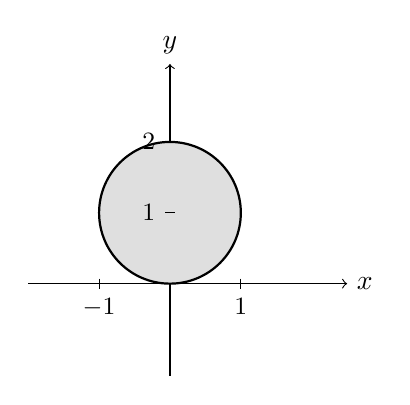
\begin{tikzpicture}[scale=0.9]
  \draw[->] (-2,0) -- (2.5,0) node[right] {$x$};
  \draw[->] (0,-1.3) -- (0,3.1) node[above] {$y$};
  \fill[gray!25] (0,1) circle (1);
  \draw[thick] (0,1) circle (1);
  \foreach \x in {-1,1} \draw (\x,2pt) -- (\x,-2pt) node[below] {\small$\x$};
  \foreach \y in {1,2} \draw (2pt,\y) -- (-2pt,\y) node[left] {\small$\y$};
\end{tikzpicture}
\end{figure}	 
La placa está representada por la figura punteada.  La integral de masa está definida por $$m=\int_{0}^{\pi}\int_{0}^{2\sen \theta}\left( r \right)\ rdrd\theta.$$
Resolviendo la integral por medio de coordenadas polares:
$\displaystyle\int_{0}^{2\sen \theta}r^2\ dr=\dfrac{r^3}{3}\Big|_{0}^{2\sen \theta}=\dfrac{\left(  2\sen\theta \right)^{3}}{3}-0=\dfrac{\left(  2\sen\theta \right)^{3}}{3}.$
\begin{align*}
\displaystyle\int_{0}^{\pi}\dfrac{8\sen^3 \theta}{3}\ d\theta&=\dfrac{8}{3}\displaystyle\int_{0}^{\pi}\sen^3 \theta\ d\theta=\dfrac{8}{3}\displaystyle\int_{0}^{\pi}\sen^2 \theta \sen \theta\ d\theta \\ 
 & =\dfrac{8}{3}\displaystyle\int_{0}^{\pi}\left( 1-\cos^2\theta \right)  \sen \theta\ d\theta=\dfrac{8}{3}\displaystyle\int_{0}^{\pi}\sen \theta\ d\theta -\dfrac{8}{3}\displaystyle\int_{0}^{\pi}\cos^2\theta  \sen \theta\ d\theta  \\ 
 &=\dfrac{-8}{3}\cos\theta \Big|_{0}^{\pi}-I.\\
\end{align*}
Resolviendo la integral $I,$ Tome $\omega=\cos \theta ,$ por lo cual $d\omega =\sen \theta\ d\theta.$ 
Esto implica que, $I=\dfrac{8}{3}\displaystyle\int \cos^2\theta  \sen \theta\ d\theta=\dfrac{8}{3}\int \omega^{2}\ d\omega=\dfrac{8}{3}\dfrac{\omega^3}{3}+C.$
Llevando este resultado a la solución del problema, $$m=\dfrac{-8}{3}\cos\theta \Big|_{0}^{\pi}-\dfrac{\cos ^3\theta}{9}\Big|_{0}^{\pi}=\dfrac{8}{3}\left[-\cos \pi +\cos 0\right]-\dfrac{8}{9}\left[\cos^3 \pi +\cos^3 0\right]=\dfrac{32}{9}. $$
Por lo cual la masa de la lámina es $m=\dfrac{32}{9}.$ 
\end{myproof}
\end{prob}

% [Original: líneas 2141-2167 | sin verificar | PSTRICKS - pendiente convertir a tikz | 2 variante(s) de parámetro (se descartaron 1)]
\begin{prob}
Considere la región $R$ (ver figura \ref{fig1.2}), la cual está limitada por las curvas $y=-x+6,$ $x^2+y^2=9$ y  $(x - 3)^{2} + y^{2} = 9.$ Use coordenadas polares para calcular la integral $\displaystyle\int\int_{R}  \dfrac{dA}{\sqrt{\left(x^2+y^2\right)^3}}$.
\begin{figure}[H]
\centering
\begin{tikzpicture}[scale=0.7]
  \draw[->] (-2,0) -- (8,0) node[right] {$x$};
  \draw[->] (0,-2.4) -- (0,5) node[above] {$y$};
  \draw[thick, red] (3,0) arc[start angle=0, end angle=60, radius=3];
  \draw[thick, blue] (3,3) arc[start angle=90, end angle=120, radius=3];
  \draw[thick, red!40!black] (3,0) -- (6,0);
  \draw[thick, green!60!black] (6,0) -- (3,3);
  \node[red, right, font=\small] at (0.4,1.7) {$x^2{+}y^2{=}9$};
  \node[blue, above, font=\small] at (0.3,4.2) {$(x{-}3)^2{+}y^2{=}9$};
  \node[green!60!black, right, font=\small] at (4.2,2.6) {$y{=}{-}x{+}6$};
  \node[below, font=\small] at (4.5,0) {$y{=}0$};
  \fill[red] (3,0) circle (3pt);
  \fill[red] (1.5,2.598) circle (3pt);
  \fill[red] (3,3) circle (3pt);
  \fill[red] (6,0) circle (3pt);
  \foreach \x in {2,4,6} \draw (\x,2pt) -- (\x,-2pt) node[below] {\tiny$\x$};
  \foreach \y in {2,4} \draw (2pt,\y) -- (-2pt,\y) node[left] {\tiny$\y$};
\end{tikzpicture}
\caption{Región del segundo ejercicio}\label{fig1.2}
\end{figure}
\end{prob}

% [Original: líneas 2295-2321 | sin verificar | PSTRICKS - pendiente convertir a tikz]
\begin{prob}
Considere la región $R$ (ver figura \ref{fig3.2}), la cual está limitada por las curvas $y=-x+10,$ $x^2+y^2=25$ y  $(x - 5)^{2} + y^{2} = 25.$ Use coordenadas polares para calcular la integral $\displaystyle\int\int_{R}  \dfrac{dA}{\sqrt{\left(x^2+y^2\right)^3}}$.
\begin{figure}[H]
\centering
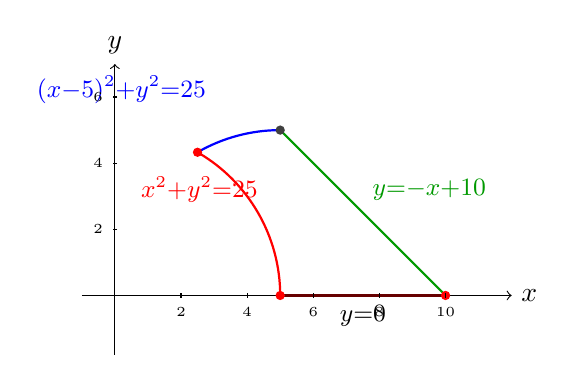
\begin{tikzpicture}[scale=0.42]
  \draw[->] (-1,0) -- (12,0) node[right] {$x$};
  \draw[->] (0,-1.8) -- (0,7) node[above] {$y$};
  \draw[thick, red] (5,0) arc[start angle=0, end angle=60, radius=5];
  \draw[thick, blue] (5,5) arc[start angle=90, end angle=120, radius=5];
  \draw[thick, red!40!black] (5,0) -- (10,0);
  \draw[thick, green!60!black] (10,0) -- (5,5);
  \node[red, right, font=\small] at (0.5,3.2) {$x^2{+}y^2{=}25$};
  \node[blue, above, font=\small] at (0.2,5.5) {$(x{-}5)^2{+}y^2{=}25$};
  \node[green!60!black, right, font=\small] at (7.5,3.2) {$y{=}{-}x{+}10$};
  \node[below, font=\small] at (7.5,0) {$y{=}0$};
  \fill[red] (5,0) circle (4pt);
  \fill[red] (2.5,4.33) circle (4pt);
  \fill[red] (10,0) circle (4pt);
  \fill[darkgray] (5,5) circle (4pt);
  \foreach \x in {2,4,6,8,10} \draw (\x,2pt) -- (\x,-2pt) node[below] {\tiny$\x$};
  \foreach \y in {2,4,6} \draw (2pt,\y) -- (-2pt,\y) node[left] {\tiny$\y$};
\end{tikzpicture}
\caption{Región del segundo ejercicio}\label{fig3.2}
\end{figure}
\end{prob}

% --- Subtema: Masa, centro de masa y momentos (18 problemas) ---

% >>> LISTOS PARA INTEGRAR AHORA <<<

% [Original: líneas 1612-1614 | sin verificar | sin figura | 5 variante(s) de parámetro (se descartaron 4)]
\begin{prob}
Determine la masa de la lámina acotada por las curvas $y=0$ y $y=\sqrt{25-x^2}$ cuya densidad está dada por la función $\delta(x,y)=y.$ Haga un bosquejo de la lámina.
\end{prob}

% [Original: líneas 1713-1720 | sin verificar | sin figura]
\begin{prob}
Una lámina cuya densidad está determinada por la función $\rho(x,y)=5x+2y+1$ tiene la forma de una región triangular cuyos vértices son los puntos $(0,0),$ $(3,3)$ y $(3,0).$ De acuerdo a la información dada:
\begin{enumerate}[(a)] 
\item Realice la gráfica de la lámina.
\item Use integrales dobles para determinar la masa de la lámina. Exprese claramente los límites de integración correspondientes y la solución de la integral.
\item Use integrales dobles para determinar el centro de masa de la lámina. Exprese claramente los límites de integración correspondientes y la solución de la integral.
\end{enumerate}
\end{prob}

% [Original: líneas 1735-1742 | sin verificar | sin figura]
\begin{prob}
Una lámina cuya densidad está determinada por la función $\rho(x,y)=5x+1$ tiene la forma de una región triangular cuyos vértices son los puntos $(0,0),$ $(9,9)$ y $(9,0).$ De acuerdo a la información dada:
\begin{enumerate}[(a)] 
\item Realice la gráfica de la lámina.
\item Use integrales dobles para determinar la masa de la lámina. Exprese claramente los límites de integración correspondientes y la solución de la integral.
\item Use integrales dobles para determinar el centro de masa de la lámina. Exprese claramente los límites de integración correspondientes y la solución de la integral.
\end{enumerate}
\end{prob}


% [Original: líneas 1779-1786 | sin verificar | sin figura]
\begin{prob}
Una lámina cuya densidad está determinada por la función $\rho(x,y)=5y+3$ tiene la forma de una región triangular cuyos vértices son los puntos $(0,0),$ $(8,8)$ y $(8,0).$ De acuerdo a la información dada:
\begin{enumerate}[(a)] 
\item Realice la gráfica de la lámina.
\item Use integrales dobles para determinar la masa de la lámina. Exprese claramente los límites de integración correspondientes y la solución de la integral.
\item Use integrales dobles para determinar el centro de masa de la lámina. Exprese claramente los límites de integración correspondientes y la solución de la integral.
\end{enumerate}
\end{prob}




% [Original: líneas 1882-1884 | sin verificar | sin figura]
\begin{prob}
Determine el centro de masa del sólido homogéneo (cuya densidad es constante) dentro de $x^2+y^2=4,$ fuera de $x^2+y^2=1,$ bajo $z=12-x^2-y^2$ y arriba de $z=0.$
\end{prob}

% [Original: líneas 2014-2030 | solución completa | sin figura]
\begin{prob}
Determine el centro de masa de la lámina de densidad $\delta(x,y)=y+1$ sobre el rectángulo $[0,4]\times[0,3]$.
\begin{myproof} 
Observe que 
\begin{align*}
M_{x}&=\int_{0}^{4}\int_{0}^{3}y\left(y+1\right)\ dydx,\\
&=\int_{0}^{3}\left(y^2+y\right)\ dy  = \dfrac{y^3}{3}+\dfrac{y^2}{2}\Big|_{0}^{3}=\dfrac{27}{2}.\\
&=\int_{0}^{3}\dfrac{27}{2}\ dx  = \dfrac{27x}{2}\Big|_{0}^{4}=54.
\end{align*}
\begin{align*}
M_{y}&=\int_{0}^{3}\int_{0}^{4}x\left(y+1\right)\ dxdy,\\
&=\int_{0}^{4}\left(xy+x\right)\ dx  = \dfrac{yx^2}{2}+\dfrac{x^2}{2}\Big|_{0}^{4}=8y+8.\\
&=\int_{0}^{3}\left( 8y+8 \right)\ dy  = \dfrac{8y^2}{2}+8y\Big|_{0}^{3}=60.
\end{align*}
Lo cual implica que el centro de masa está en el punto $\left( \overline{x},\overline{y} \right)=\left(  \dfrac{M_y}{m},\dfrac{M_x}{m} \right)=\left(  \dfrac{60}{30},\dfrac{54}{30} \right)=\left(  2,\dfrac{9}{5} \right).$
\end{myproof}
\end{prob}

% [Original: líneas 2173-2175 | sin verificar | sin figura]
\begin{prob}
Calcule el centro de masa y los radios de giro respecto al eje $x$ y $y$ de la lámina acotada por la curva $y=\sen x$ y la recta $y=\dfrac{2x}{\pi}$ cuya densidad está dada por $\rho(x,y)=2+x+y.$ Construya la gráfica de la región que determina la lámina.
\end{prob}

% [Original: líneas 2239-2241 | sin verificar | sin figura]
\begin{prob}
Calcule el centro de masa y los radios de giro respecto al eje $x$ y $y$ de la lámina acotada por la curva $y=\cos x$ y la recta $y=1-\dfrac{2x}{\pi}$ cuya densidad está dada por $\rho(x,y)=3+x+y.$ Construya la gráfica de la región que determina la lámina.
\end{prob}


% [Original: líneas 2327-2329 | sin verificar | sin figura]
\begin{prob}
Calcule el centro de masa y los radios de giro respecto al eje $x$ y $y$ de la lámina acotada por la curva $y=\sen x$ y la recta $y=2-\dfrac{2x}{\pi}$ cuya densidad está dada por $\rho(x,y)=1+x+y.$ Construya la gráfica de la región que determina la lámina.
\end{prob}

% [Original: líneas 2351-2359 | solo respuesta final | sin figura | 3 variante(s) de parámetro (se descartaron 2)]
\begin{prob}
Plantee las integrales que permiten calcular la masa y los momentos de masa respecto a los planos $xy,$ $yz$ y $xz$ del sólido $S$ en el primer octante, dentro de la esfera $x^2+y^2+z^2=25$ y fuera de la esfera $x^2+y^2+z^2=16,$ cuya densidad es proporcional a la distancia desde el origen. \textbf{Use un CAS para calcular el valor de cada integral.} Adjunte la captura de pantalla del programa utilizado con la solución dada. (Sugerencia: Algunos CAS gratuitos son \textit{WolframAlpha}\textregistered , \textit{Symbolab}\textregistered , o \textit{Photomath}\textregistered. )\footnote{Los vínculos web son \url{https://www.wolframalpha.com}, \url{https://es.symbolab.com}, \url{https://photomath.net/es/}}
\textbf{Respuestas:} Sea $k$ la constante de proporcionalidad, entonces: \begin{enumerate}
    \item $m\approx (144.906)k .$
    \item $M_{xy}\approx (330.0243)k .$
    \item $M_{yz}\approx (330.0243)k .$
    \item $M_{xz}\approx (330.0243)k  .$
\end{enumerate}
\end{prob}

% >>> ESPERAN PASADA CON CLAUDE CODE (pstricks) <<<

% [Original: líneas 1564-1590 | solución completa | PSTRICKS - pendiente convertir a tikz]
\begin{prob}
Determine la masa de la lámina acotada por las curvas $x=0,\ x=4,\ y=0,\ y=3,$ cuya densidad está dada por la función $\rho(x,y)=y+1.$
\begin{myproof} 
\begin{figure}[H]
\centering
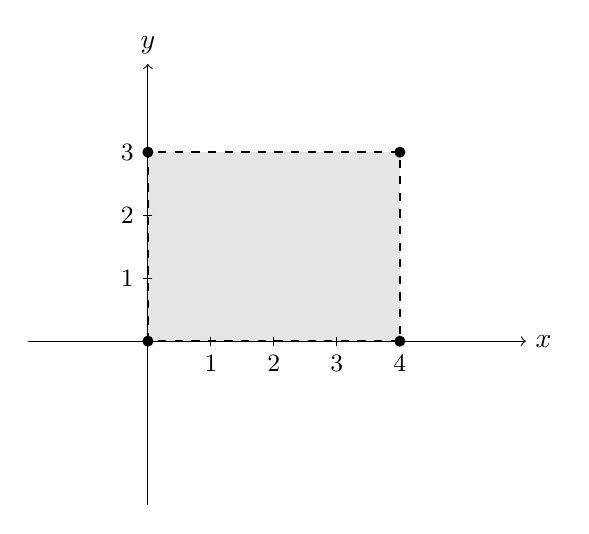
\begin{tikzpicture}[scale=0.8]
  \draw[->] (-1.9,0) -- (6,0) node[right] {$x$};
  \draw[->] (0,-2.6) -- (0,4.4) node[above] {$y$};
  \fill[gray!20] (0,0) rectangle (4,3);
  \draw[thick, dashed] (0,0) rectangle (4,3);
  \fill (4,0) circle (2.5pt); \fill (0,3) circle (2.5pt);
  \fill (4,3) circle (2.5pt); \fill (0,0) circle (2.5pt);
  \foreach \x in {1,2,3,4} \draw (\x,2pt) -- (\x,-2pt) node[below] {\small$\x$};
  \foreach \y in {1,2,3} \draw (2pt,\y) -- (-2pt,\y) node[left] {\small$\y$};
\end{tikzpicture}
\end{figure}	 
La placa está representada por la figura punteada. La integral de masa está definida por $$m=\int_{0}^{4}\int_{0}^{3}\left( y+1 \right)\ dydx.$$
Resolviendo la integral:
$\displaystyle\int_{0}^{3}y+1\ dy=\dfrac{y^2}{2}+y\Big|_{0}^{3}=\dfrac{3^2}{2}+3-0=\dfrac{15}{2}.$
$\displaystyle\int_{0}^{4}\dfrac{15}{2}\ dx=\dfrac{15x}{2}+y\Big|_{0}^{4}=\dfrac{15(4)}{2}-0=30.$ Por lo cual la masa de la lámina es $m=30.$	
\end{myproof}
\end{prob}

% [Original: líneas 2032-2076 | solución completa | PSTRICKS - pendiente convertir a tikz]
\begin{prob}
Halle la masa $m$ y el centro de masa para la lámina acotada por $y=e^x,y=0,x=0,x=1$ cuya densidad está dada por la función $\rho (x,y)=2-x+y.$
\begin{myproof}
\begin{figure}[H]
\centering
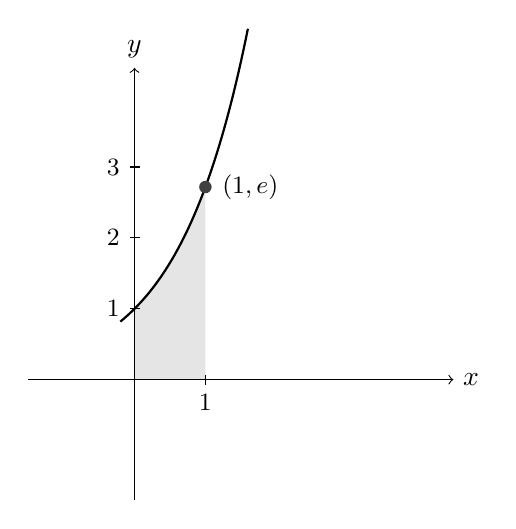
\begin{tikzpicture}[scale=0.9]
  \fill[gray!20] (0,0) -- plot[domain=0:1, samples=50] (\x,{exp(\x)}) -- (1,0) -- cycle;
  \draw[thick] plot[domain=-0.2:1.6, samples=60] (\x,{exp(\x)});
  \draw[->] (-1.5,0) -- (4.5,0) node[right] {$x$};
  \draw[->] (0,-1.7) -- (0,4.4) node[above] {$y$};
  \fill[darkgray] (1,{exp(1)}) circle (2.5pt);
  \node[right, font=\small] at (1.1,{exp(1)}) {$(1,e)$};
  \draw (1,2pt) -- (1,-2pt) node[below] {\small$1$};
  \foreach \y in {1,2,3} \draw (2pt,\y) -- (-2pt,\y) node[left] {\small$\y$};
\end{tikzpicture}
\end{figure}
La placa está representada por la figura rayada.  La integral de masa está definida por $$m=\int_{0}^{1}\int_{0}^{e^x}\left( 2-x+y\right)\ dydx.$$
Resolviendo la integral:
$\displaystyle\int_{0}^{e^x}(2-x+y)\ dy=2y-xy+\dfrac{y^2}{2}\Big|_{0}^{e^x}=2e^x-xe^x+\dfrac{e^{2x}}{2}.$
\begin{align*}
&\displaystyle\int_{0}^{1}\left( 2e^x-xe^x+\dfrac{e^{2x}}{2} \right)\ dx\\
=&\displaystyle\int_{0}^{1}2e^{x}\ dx  - \displaystyle\int_{0}^{1}xe^{x}\ dx+\displaystyle\int_{0}^{1} \dfrac{e^{2x}}{2}\ dx\\ &=\left[2e^x-(x-1)e^x+\dfrac{e^{2x}}{4}\right]\Big|_{0}^{1} \\ 
& =\dfrac{e^2+8e-13}{4}.
\end{align*}
Por lo cual, $m=\dfrac{e^2+8e-13}{4}.$ 
\textbf{Nota:} La integral $\displaystyle\int xe^{x}dx=(x-1)e^x+C$ se obtiene haciendo integración por partes.
Ahora, observe que 
\begin{align*}
M_{x}&=\int_{0}^{1}\int_{0}^{e^x}y\left(2-x+y\right)\ dydx,\\
&=\int_{0}^{e^x}\left(2y-xy+y^2\right)\ dy  \\ &=\dfrac{2y^2}{2}-\dfrac{xy^2}{2}+\dfrac{y^3}{3}\Big|_{0}^{e^x}\\&=e^{2x}-xe^{2x}+\dfrac{e^{3x}}{3}.\\
&=\int_{0}^{1} \left( e^{2x}-xe^{2x}+\dfrac{e^{3x}}{3} \right) \ dx  \\
&= \dfrac{e^{2x}}{2}-\dfrac{1}{4}e^{2x}\left( 2x-1 \right)+\dfrac{e^{3x}}{9}\Big|_{0}^{1}\\
&=\dfrac{8e^3+27e^2-53}{72}.
\end{align*}
\textbf{Nota:} La integral $\displaystyle\int xe^{2x}dx=\dfrac{1}{4}e^{2x}(2x-1)+C$ se obtiene haciendo integración por partes.
\begin{align*}
M_{y}&=\int_{0}^{1}\int_{0}^{e^x}x\left(2-x+y\right)\ dydx,\\
&=\int_{0}^{e^x}\left(2x-x^2+xy\right)\ dy  \\ &=2xy-x^2y+\dfrac{xy^2}{2}\Big|_{0}^{e^x}\\&=2xe^{x}-x^2e^{x}+\dfrac{xe^{2x}}{2}.\\
&=\int_{0}^{1} \left( 2xe^{x}-x^2e^{x}+\dfrac{xe^{2x}}{2} \right) \ dx  \\
&=2(x-1)e^{x}-(x^2-2x+2)e^x+ \dfrac{1}{8}\left( 2x-1 \right)e^{2x}\Big|_{0}^{1}\\
&=\dfrac{e^2-8e+33}{8}.
\end{align*}
\textbf{Nota:} La integral $\displaystyle\int x^2e^{x}dx=(x^2-2x+2)e^x+C$ se obtiene haciendo integración por partes.
Lo cual implica que el centro de masa está en el punto $$\left( \overline{x},\overline{y} \right)=\left(  \dfrac{M_y}{m},\dfrac{M_x}{m} \right)=\left(  \dfrac{ \dfrac{e^2-8e+33}{8}  }{ \dfrac{e^2+8e-13}{4} },\dfrac{  \dfrac{8e^3+27e^2-53}{72}}{\dfrac{e^2+8e-13}{4}} \right)\approx\left( 0.577  , 1.058 \right).$$
\end{myproof}
\end{prob}

% [Original: líneas 2078-2114 | solución completa | PSTRICKS - pendiente convertir a tikz]
\begin{prob}
Verifique que los momentos de inercia de una lámina rectangular, con ancho $b$, altura $h$ y densidad $\rho(x,y)=1$ están dados por $I_x=\dfrac{1}{3}bh^3$ e $I_y=\dfrac{1}{3}b^3h.$ Calcule $\overline{\overline{x}}$ e $\overline{\overline{y}}.$ Vea la figura.
\begin{figure}[H]
\centering
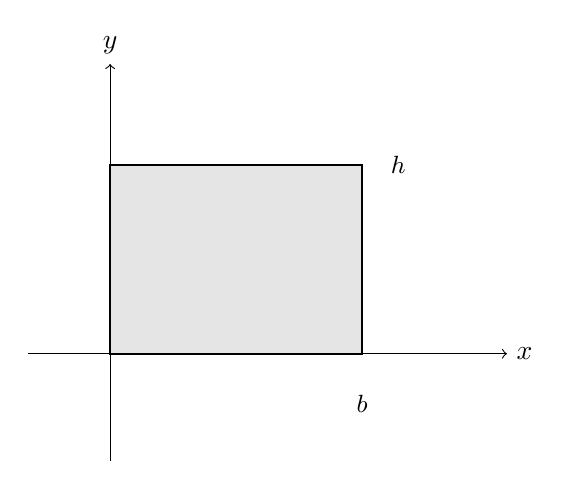
\begin{tikzpicture}[scale=0.8]
  \draw[->] (-1.3,0) -- (6.3,0) node[right] {$x$};
  \draw[->] (0,-1.7) -- (0,4.6) node[above] {$y$};
  \fill[gray!20] (0,0) rectangle (4,3);
  \draw[thick] (0,0) rectangle (4,3);
  \node[below, font=\small] at (4,-0.5) {$b$};
  \node[right, font=\small] at (4.3,3) {$h$};
\end{tikzpicture}
\end{figure}
\begin{myproof}
Observe que la masa de la lámina está dada por $$m=\int_{0}^{h}\int_{0}^{b}1\ dydx$$
Calculando la integral,
\begin{align*}
\int_{0}^{b}dx&=x\Big|_{0}^{b}=b\\
&=\int_{0}^{h}b\ dy=by\Big|_{0}^{h}=bh.
\end{align*}
Las integrales de los momentos de inercia resultan en $I_{x}=\displaystyle\int_{0}^{h}\int_{0}^{b} y^2\ dxdy$ y $I_{y}=\displaystyle\int_{0}^{h}\int_{0}^{b} x^2\ dxdy.$
Calculando las integrales:
 \begin{align*}
 I_x&=\int_{0}^{b}y^2\ dx=y^2x\Big|_{0}^{b}=y^2b,\\
 &=\int_{0}^{h}y^2b\ dy=b\dfrac{y^3}{3}\Big|_{0}^{h}=\dfrac{bh^3}{3}.
 \end{align*}
 \begin{align*}
 I_y=&\int_{0}^{b}x^2\ dx=\dfrac{x^3}{3}\Big|_{0}^{b}=\dfrac{b^3}{3},\\
 &=\int_{0}^{h}\dfrac{b^3}{3}\ dy=y\dfrac{b^3}{3}\Big|_{0}^{h}=\dfrac{hb^3}{3}.
 \end{align*}
Finalmente, el radio de giro en $X$ está dado por $\overline{\overline{x}}=\sqrt{\dfrac{\dfrac{b^3h}{3}}{bh}}=\sqrt{\dfrac{b^2}{3}}$
  y el radio de giro en $Y,$ $\overline{\overline{y}}=\sqrt{\dfrac{\dfrac{h^3b}{3}}{bh}}=\sqrt{\dfrac{h^2}{3}}.$	
\end{myproof}
\end{prob}

% --- Subtema: Volumen / área (coordenadas rectangulares) (18 problemas) ---

% >>> LISTOS PARA INTEGRAR AHORA <<<

% [Original: líneas 1484-1486 | sin verificar | sin figura | 3 variante(s) de parámetro (se descartaron 2)]
\begin{prob}
Calcule el volumen del sólido $Q$ limitado por las superficies $z=\dfrac{y}{x^2+9},$ $x^2+y^2=9$ cuando $x\geq 0$ y $y\geq 0.$ 
\end{prob}

% [Original: líneas 1608-1610 | sin verificar | sin figura | 5 variante(s) de parámetro (se descartaron 4)]
\begin{prob}
Determine el área de la región dentro de la circunferencia $x^2+(y-5)^2=25$ y fuera de la circunferencia $x^2+y^2=25.$ Haga un bosquejo de la región.
\end{prob}

% [Original: líneas 1616-1618 | sin verificar | sin figura]
\begin{prob}
Determine el volumen del tetraedro acotado por los planos de coordenadas y el plano $x+5y+z=5.$
\end{prob}

% [Original: líneas 1620-1622 | sin verificar | sin figura | 6 variante(s) de parámetro (se descartaron 5)]
\begin{prob}
Calcule el volumen del sólido acotado por el plano $z=0$ y el paraboloide $z=25-x^2-y^2.$ 
\end{prob}

% [Original: líneas 1639-1641 | sin verificar | sin figura | 3 variante(s) de parámetro (se descartaron 2)]
\begin{prob}
Determine el volumen del tetraedro acotado por los planos de coordenadas y el plano $4x+3y+z=12.$
\end{prob}

% [Original: líneas 1662-1664 | sin verificar | sin figura | 2 variante(s) de parámetro (se descartaron 1)]
\begin{prob}
Determine el volumen del tetraedro acotado por los planos de coordenadas y el plano $2x+y+z=2.$
\end{prob}

% [Original: líneas 1886-1892 | sin verificar | sin figura]
\begin{prob}
Considere el sólido acotado por la superficie $z=16-x^2-y^2$ y los planos de coordenadas $x=0,$ $y=0$ y $z=0.$
\begin{enumerate}[(a)]     
    \item Plantee una integral doble que permita calcular el volumen del sólido propuesto.
    \item Resuelva la integral que planteó en el ítem anterior. Si hace algún cambio de variable, exprese claramente la definición de los nuevos límites de integración. Muestre explícitamente cada uno de los cálculos realizados en la solución de la integral.
\end{enumerate}    
\end{prob}

% [Original: líneas 1921-1923 | sin verificar | sin figura | 2 variante(s) de parámetro (se descartaron 1)]
\begin{prob}
Use integrales dobles o triples para calcular el volumen del sólido acotado por el plano $z=0$ y el paraboloide $z=9-x^2-y^2.$ Determine explícitamente los límites de integración y si realiza algún cambio de coordenadas exprese claramente los nuevos límites correspondientes.
\end{prob}

% [Original: líneas 2169-2171 | sin verificar | sin figura | 2 variante(s) de parámetro (se descartaron 1)]
\begin{prob}
Demuestre que las áreas superficiales de los paraboloides $x^2+y^2=6z$ y $x^2-y^2=6z$ sobre la región $R=\left\lbrace (x,y):\ x^2+y^2=16 \right\rbrace$ miden lo mismo. Calcule tal área.
\end{prob}


% [Original: líneas 2347-2349 | solo respuesta final | sin figura]
\begin{prob}
Calcule el volumen del sólido acotado por $z=x^2+y^2,$ $z=0,$ y $(x-1)^2+y^2=1.$ (Sugerencia: Use un CAS para observar el sólido). \textbf{Respuesta:} $\approx  4.12738$.
\end{prob}

% [Original: líneas 2373-2375 | solo respuesta final | sin figura]
\begin{prob}
Calcule el volumen del sólido acotado por $z=x^2+y^2,$ $z=0,$ y $x^2+(y-4)^2=16.$ (Sugerencia: Use un CAS para observar el sólido). \textbf{Respuesta:} $\approx 1206.3715$.
\end{prob}

% [Original: líneas 2399-2401 | solo respuesta final | sin figura]
\begin{prob}
Calcule el volumen del sólido acotado por $z=2x^2+2y^2,$ $z=0,$ y $x^2+(y-1)^2=1.$ (Sugerencia: Use un CAS para observar el sólido). \textbf{Respuesta:} $\approx 9.42477$.
\end{prob}

% >>> ESPERAN PASADA CON CLAUDE CODE (pstricks) <<<

% [Original: líneas 1454-1478 | sin verificar | PSTRICKS - pendiente convertir a tikz | 3 variante(s) de parámetro (se descartaron 2)]
\begin{prob}
Considere la región $R$ (ver figura \ref{fig1.1}), la cual está limitada por las curvas $y=x+5,$ $y=-x^2-4x-1,$ $y=x-1,$ $y=5x^2-10x+5.$ Plantee la integral doble que permite calcular el área encerrada por estas curvas y determine el valor de esta área.
\begin{figure}[H]\centering
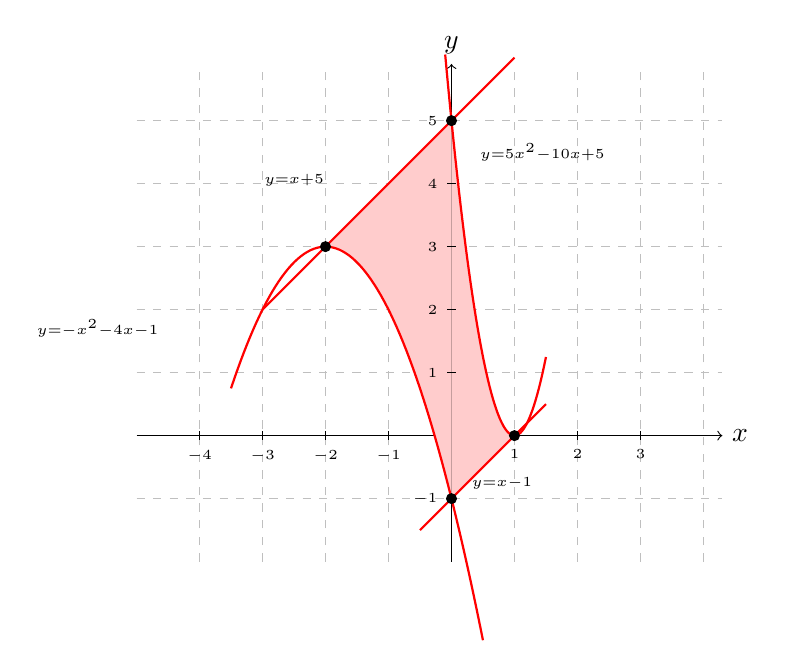
\begin{tikzpicture}[scale=0.8]
  \draw[->] (-5,0) -- (4.3,0) node[right] {$x$};
  \draw[->] (0,-2) -- (0,5.9) node[above] {$y$};
  \foreach \gx in {-4,-3,-2,-1,1,2,3,4} \draw[lightgray, dashed, thin] (\gx,-2) -- (\gx,5.9);
  \foreach \gy in {-1,1,2,3,4,5} \draw[lightgray, dashed, thin] (-5,\gy) -- (4.3,\gy);
  \fill[red!20]
    plot[domain=-2:0, samples=30] (\x,{-\x*\x-4*\x-1})
    -- (0,5)
    -- plot[domain=0:-2, samples=30] (\x,{\x+5})
    -- cycle;
  \fill[red!20]
    plot[domain=0:1, samples=20] (\x,{\x-1})
    -- plot[domain=1:0, samples=20] (\x,{5*\x*\x-10*\x+5})
    -- (0,-1)
    -- cycle;
  \draw[thick, red] plot[domain=-3.5:0.5, samples=80] (\x,{-\x*\x-4*\x-1});
  \draw[thick, red] plot[domain=-3:1, samples=60] (\x,{\x+5});
  \draw[thick, red] plot[domain=-0.1:1.5, samples=60] (\x,{5*\x*\x-10*\x+5});
  \draw[thick, red] plot[domain=-0.5:1.5, samples=40] (\x,{\x-1});
  \node[left, font=\tiny] at (-4.5,1.7) {$y{=}{-}x^2{-}4x{-}1$};
  \node[right, font=\tiny] at (0.3,4.5) {$y{=}5x^2{-}10x{+}5$};
  \node[above, font=\tiny] at (-2.5,3.8) {$y{=}x{+}5$};
  \node[below, font=\tiny] at (0.8,-0.5) {$y{=}x{-}1$};
  \foreach \x in {-4,-3,-2,-1,1,2,3} \draw (\x,2pt) -- (\x,-2pt) node[below, font=\tiny] {$\x$};
  \foreach \y in {-1,1,2,3,4,5} \draw (2pt,\y) -- (-2pt,\y) node[left, font=\tiny] {$\y$};
  \fill (0,5) circle (2.5pt); \fill (1,0) circle (2.5pt);
  \fill (-2,3) circle (2.5pt); \fill (0,-1) circle (2.5pt);
\end{tikzpicture}
\caption{Región del primer ejercicio}\label{fig1.1}
\end{figure}
Respuesta: 41/6.
\end{prob}



% [Original: líneas 1925-1947 | sin verificar | PSTRICKS - pendiente convertir a tikz]
\begin{prob}
Considere la región $R$ (ver la figura), la cual está limitada por las curvas $y=2x+4,$ $y=-2x^2-4x,$ $y=3x,$ $y=-x^2+4.$ 
\begin{enumerate}[(a)]
\item Plantee la integral doble que permite calcular el área encerrada por estas curvas. Defina claramente los límites de integración.
\item Evalúe la integral que obtuvo en el paso anterior. Muestre explícitamente todos los cálculos necesarios para obtener el área.
\end{enumerate}
\begin{figure}[H]
\centering
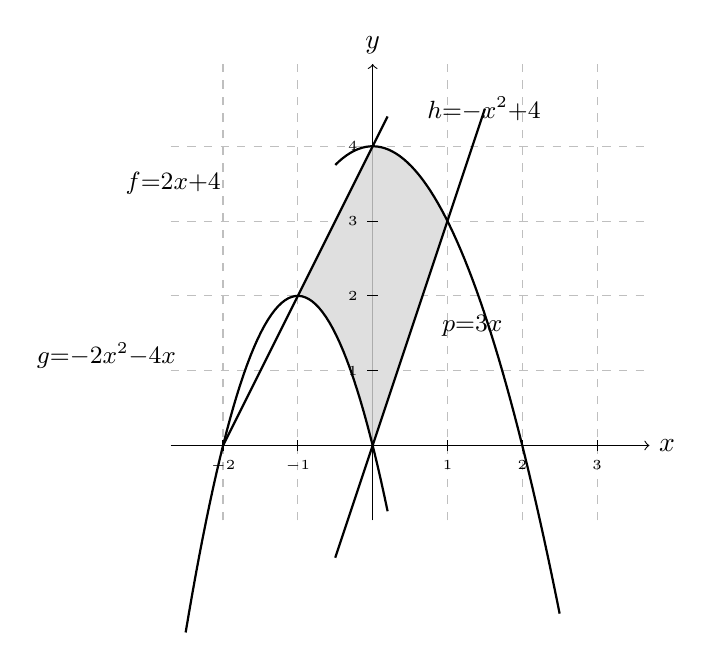
\begin{tikzpicture}[scale=0.95]
  \draw[->] (-2.7,0) -- (3.7,0) node[right] {$x$};
  \draw[->] (0,-1) -- (0,5.1) node[above] {$y$};
  \foreach \gx in {-2,-1,1,2,3} \draw[lightgray, dashed, thin] (\gx,-1) -- (\gx,5.1);
  \foreach \gy in {1,2,3,4} \draw[lightgray, dashed, thin] (-2.7,\gy) -- (3.7,\gy);
  \fill[gray!25]
    plot[domain=-1:0, samples=20] (\x,{2*\x+4})
    -- (0,0)
    -- plot[domain=0:-1, samples=20] (\x,{-2*\x*\x-4*\x})
    -- cycle;
  \fill[gray!25]
    plot[domain=0:1, samples=20] (\x,{3*\x})
    -- plot[domain=1:0, samples=20] (\x,{-\x*\x+4})
    -- (0,0)
    -- cycle;
  \draw[thick] plot[domain=-2:0.2, samples=60] (\x,{2*\x+4});
  \draw[thick] plot[domain=-2.5:0.2, samples=60] (\x,{-2*\x*\x-4*\x});
  \draw[thick] plot[domain=-0.5:2.5, samples=60] (\x,{-\x*\x+4});
  \draw[thick] plot[domain=-0.5:1.5, samples=30] (\x,{3*\x});
  \node[left, font=\small] at (-1.9,3.5) {$f{=}2x{+}4$};
  \node[left, font=\small] at (-2.5,1.2) {$g{=}{-}2x^2{-}4x$};
  \node[right, font=\small] at (0.6,4.5) {$h{=}{-}x^2{+}4$};
  \node[right, font=\small] at (0.8,1.6) {$p{=}3x$};
  \foreach \x in {-2,-1,1,2,3} \draw (\x,2pt) -- (\x,-2pt) node[below, font=\tiny] {$\x$};
  \foreach \y in {1,2,3,4} \draw (2pt,\y) -- (-2pt,\y) node[left, font=\tiny] {$\y$};
\end{tikzpicture}
\caption{Figura para el problema 1.}
\end{figure}
\end{prob}


% --- Subtema: Verdadero o falso (6 problemas) ---

% >>> LISTOS PARA INTEGRAR AHORA <<<

% [Original: líneas 1624-1629 | sin verificar | sin figura | 5 variante(s) de parámetro (se descartaron 4)]
\begin{prob}
Determine si la siguiente afirmación es falsa o verdadera. Justifique su respuesta.
\begin{center}
{\fboxrule=.3pt \fboxsep=3pt\fbox{ Si $B=\left\lbrace \left(x,y,z \right)\in \mathbb{R}^3 : x^2+y^2+z^2\leq  9 \right\rbrace,$ entonces $\displaystyle\int\int\int_{B}\ dV=36\pi.$ }}        
\end{center}   
\end{prob}

% [Original: líneas 1706-1711 | sin verificar | sin figura | 5 variante(s) de parámetro (se descartaron 4)]
\begin{prob}
Determine si la siguiente afirmación es falsa o verdadera. Justifique su respuesta convenientemente, respuesta sin justificar no vale.
\begin{center}     
{\fboxrule=.3pt \fboxsep=3pt\fbox{ Si $R$ es la región del plano determinada por el círculo $x^2+y^2=9$, entonces $\displaystyle\int\int_{R}\ 5\ dA= 90\pi .$ }}        
\end{center} 
\end{prob}

% [Original: líneas 1728-1733 | sin verificar | sin figura | 3 variante(s) de parámetro (se descartaron 2)]
\begin{prob}
Determine si la siguiente afirmación es falsa o verdadera. Justifique su respuesta convenientemente, respuesta sin justificar no vale.
\begin{center}
{\fboxrule=.3pt \fboxsep=3pt\fbox{ Si $R$ es la región del plano determinada por el círculo $x^2+y^2=81$, entonces $\displaystyle\int\int_{R}\ 8\ dA= 648\pi .$ }}        
\end{center} 
\end{prob}

% [Original: líneas 1910-1915 | sin verificar | sin figura | 2 variante(s) de parámetro (se descartaron 1)]
\begin{prob}
Determine si la siguiente afirmación es falsa o verdadera. Justifique su respuesta convenientemente, respuesta sin justificar no vale.
\begin{center}
{\fboxrule=.3pt \fboxsep=3pt\fbox{ Si $B$ representa  a una esfera de radio $3$ en $\mathbb{R}^3$, entonces $\displaystyle\int\int\int_{B}\ dV= 108\pi .$ }}        
\end{center}   
\end{prob}

% [Original: líneas 2273-2278 | sin verificar | sin figura]
\begin{prob}
Determine si la siguiente afirmación es falsa o verdadera. Justifique su respuesta convenientemente, respuesta sin justificar no vale.
\begin{center}     
{\fboxrule=.3pt \fboxsep=3pt\fbox{ Si $B$ representa  a la esfera $x^2+y^2+z^2=4$ en $\mathbb{R}^3$, entonces $\displaystyle\int\int\int_{B}\ dV=\dfrac{256\pi}{3}.$ }}        
\end{center} 
\end{prob}

% [Original: líneas 2467-2472 | sin verificar | sin figura]
\begin{prob}
Determine si la siguiente afirmación es falsa o verdadera. Justifique su respuesta.
\begin{center}     
{\fboxrule=.3pt \fboxsep=3pt\fbox{ Si $B=\left\lbrace \left(x,y,z \right)\in \mathbb{R}^3 : x^2+y^2+z^2\leq  25 \right\rbrace,$ entonces $\displaystyle\int\int\int_{B}\ 6dV=1000\pi.$ }}        
\end{center}   
\end{prob}

% --- Subtema: Otros (9 problemas) ---

% >>> LISTOS PARA INTEGRAR AHORA <<<

% [Original: líneas 1492-1494 | sin verificar | sin figura]
\begin{prob}
Calcule  la  integral triple $$\displaystyle\int\int\int_{\Omega}x^2\  dV,$$ donde $\Omega$ es la región acotada por las curvas $x^2+z=1,$  $y^2+z=1$ y el plano $xy$.
\end{prob}

% [Original: líneas 1534-1536 | sin verificar | sin figura | 2 variante(s) de parámetro (se descartaron 1)]
\begin{prob}
Calcule  la  integral triple $$\displaystyle\int\int\int_{\Omega}z\  dV,$$ donde $\Omega$ es la región acotada por las curvas $x^2+z=1,$  $y^2+z=1$ y el plano $xy$.
\end{prob}


% [Original: líneas 1917-1919 | sin verificar | sin figura | 2 variante(s) de parámetro (se descartaron 1)]
\begin{prob}
Considere la región triangular $S$ con vértices $(0,0),$ $(3,0),$ y $(3,6).$ Haga una gráfica de la región descrita y calcule el valor de la integral $\displaystyle\iint_{S}8\ dA.$
\end{prob}



% [Original: líneas 2395-2397 | solo respuesta final | sin figura]
\begin{prob}
Calcule  la  integral triple $$\displaystyle\int\int\int_{\Omega}y^2\  dV,$$ donde $\Omega$ es la región acotada por las curvas $x^2+z=1,$  $y^2+z=1$ y el plano $xy$. \textbf{Respuesta:} $\approx 0.2222$.
\end{prob}

